\documentclass[12pt,a4paper]{article}
\usepackage[utf8]{inputenc}
\usepackage[shortlabels]{enumitem}
%Set page layout parameters
\usepackage[
top=4cm,
bottom=2cm,
left=2cm,
right=2cm,
headheight=2cm,
footskip=1cm,
marginparwidth=2cm]{geometry}
\usepackage{amsmath}
\usepackage[dvipsnames]{xcolor}
% To use color boxes
\usepackage{tcolorbox}
\usepackage{lipsum}
\tcbuselibrary{listings,theorems,skins,vignette,raster,breakable,magazine,poster,fitting,hooks}
\newcounter{ejemplo}
%Images path
\graphicspath{{images/}}
\usepackage{float} %provide us with the option H
\usepackage{fancyhdr}
\usepackage{tikz}
\usepackage{tikzpagenodes}
%to redefine figure caption 
\renewcommand{\figurename}{Figura}
%change text font
\usepackage[T1]{fontenc}
\usepackage{tgbonum} % LaTeX will use the TEX Gyre Bonum font family

\definecolor{subtitle_yellow}{RGB}{252,213,129}
\definecolor{title_yellow}{RGB}{249,175,16}
\definecolor{steel_blue_title}{RGB}{93,138,168}
\definecolor{pewter_blue_subtitle}{RGB}{149,178,198}
\definecolor{ecru_circle}{RGB}{215,190,130}
\definecolor{ecru_circle1}{RGB}{68,148,173}

\newcommand{\myfirststyle}{%
	\begin{tikzpicture}[remember picture, overlay]
		
		%top border
		\fill[fill=steel_blue_title](current page.north west) rectangle ([yshift=-15mm]current page.north east);
		
		\fill[fill=pewter_blue_subtitle]([yshift=-17mm]current page.north west) rectangle ([yshift=-30mm]current page.north east);
		
		%page box
		%\draw[lightgray, fill=Rhodamine, fill opacity=0.05, line width=1mm, rounded corners=3mm] ([xshift=-5mm,yshift=5mm]current page text area.north west) rectangle ([xshift=5mm,yshift=-5mm]current page text area.south east);
		
		%bottom box
		\fill[fill=pewter_blue_subtitle](current page.south west) rectangle ([yshift=10mm]current page.south east);
		
		%page circle
		\draw[white,fill=ecru_circle1,line width=2mm] ([xshift=-5mm,yshift=25mm]current page text area.north east) circle (1); 
		
		
		%page number text        
		%\node[anchor=center] at ([xshift=-5mm,yshift=25mm]current page text area.north east) {\Huge\bfseries\sffamily\color{white}{\thepage}};
		
		%title text
		\node[anchor=west] at ([yshift=32mm]current page text area.north west) {\Huge\bfseries\sffamily\color{white}{Análisis del amplificador logarítmico}};
		
		%subtitle text
		\node[anchor=west] at ([xshift=10mm,yshift=16mm]current page text area.north west) {\Large\bfseries\sffamily\color{white}{y el amplificador antilogarítmico}};
		
		%footer text
		\node[anchor=center] at ([yshift=-15mm]current page text area.south) {\large\bfseries\sffamily\color{white}{Created by: Rodrigo Castillejos}};
		
	\end{tikzpicture}
}


%create page style
\fancypagestyle{MyFirstStyle}{%
	\fancyhf{}
	\fancyhead[C]{\myfirststyle}
	\renewcommand{\headrulewidth}{0pt}
}%

\pagestyle{MyFirstStyle}

\colorlet{colexam}{red!75!black}
\newtcolorbox[use counter=ejemplo]{myexample}{%
	empty,title={Ejemplo \thetcbcounter},attach boxed title to top left,
	boxed title style={empty,size=minimal,toprule=2pt,top=4pt,
		overlay={\draw[colexam,line width=2pt]
			([yshift=-1pt]frame.north west)--([yshift=-1pt]frame.north east);}},
	coltitle=colexam,fonttitle=\Large\bfseries,
	before=\par\medskip\noindent,parbox=false,boxsep=0pt,left=0pt,right=3mm,top=4pt,
	breakable,pad at break*=0mm,vfill before first,
	overlay unbroken={\draw[colexam,line width=1pt]
		([yshift=-1pt]title.north east)--([xshift=-0.5pt,yshift=-1pt]title.north-|frame.east)
		--([xshift=-0.5pt]frame.south east)--(frame.south west); },
	overlay first={\draw[colexam,line width=1pt]
		([yshift=-1pt]title.north east)--([xshift=-0.5pt,yshift=-1pt]title.north-|frame.east)
		--([xshift=-0.5pt]frame.south east); },
	overlay middle={\draw[colexam,line width=1pt] ([xshift=-0.5pt]frame.north east)
		--([xshift=-0.5pt]frame.south east); },
	overlay last={\draw[colexam,line width=1pt] ([xshift=-0.5pt]frame.north east)
		--([xshift=-0.5pt]frame.south east)--(frame.south west);},%
}


\begin{document}
	La conversión de una señal a su valor logarítmico equivalente involucra una operación no lineal. Muchos de los conceptos de los circuitos lineales son irrelevantes en el uso de amplificadores logarítmicos. Por ejemplo, la ganancia incremental de un amplificador logarítmico ideal tiende a menos infinito conforme la entrada tiende a cero.
	
	Si consideramos la ecuación $y=log(x)$ encontramos que cada vez que $X$ sea multiplicado or una constante $A$, $Y$ se incrementa por otra constante $A_1$. Así, si $log(K) = K_1$, entonces $log(AK) = K_1 + A_1$, $log(A^{2}K) = 2A_1 + K_1$, y $log(K/A) = K_1 - A_1$. Esto proporciona una gráfica como se muestra en la figura 1.  
	\begin{figure}[H]
		\centering
		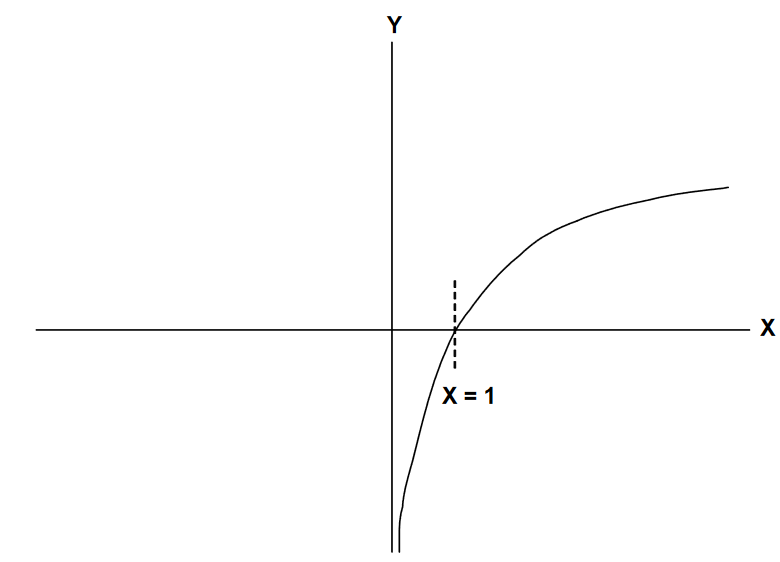
\includegraphics[scale=0.7]{log}
		\caption{Gráfica de $y = log(x)$}
		\label{fig:pic1}
	\end{figure}

	El circuito de amplificador logarítmico más fundamental se muestra en la figura \ref{fig:log_amp}. La corriente de colector $i_C$ es igual a la forma de un diodo ideal
	\begin{equation}
		i_C = I_S\left[ e^{ \frac{v_{BE}}{V_T} } - 1 \right]
	\end{equation}
	El parámetro $I_S$ es la \textbf{corriente de saturación del transistor}. Esto es, la corriente de saturación del transistor bipolar. $I_S$ es proporcional al área de sección transversal de la región de base activa del transistor, y puede tener un amplio rango de valores:
	\begin{align}
		10^{-18} A \leq I_S \leq 10^{-9} A\nonumber 
	\end{align}
	En la ecuación (1), $V_T$ es el voltaje térmico y está dado por $V_T = kT/q \simeq 0.025V$ a temperatura ambiente. 
	
	\begin{figure}[H]
		\centering
		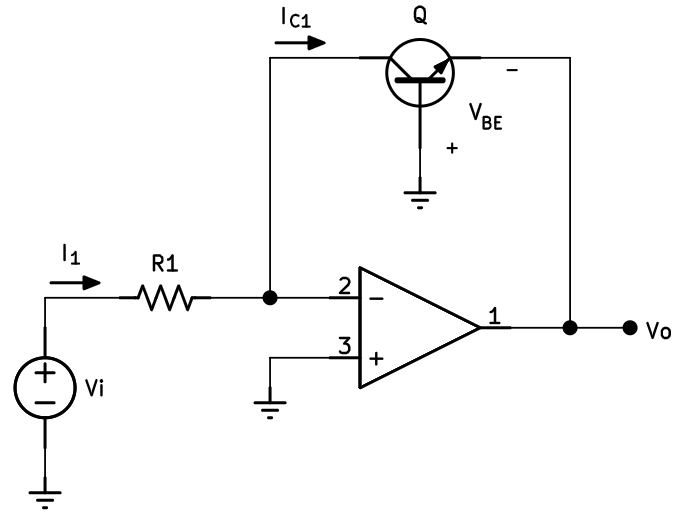
\includegraphics[scale=0.7]{log_amp}
		\caption{Amplificador logarítmico fundamental}
		\label{fig:log_amp}
	\end{figure}
	
	Debido a la muy baja corriente de saturación es posible eliminar el término constante, por o tanto
	\begin{align}
		i_C = I_S \, e^{ \frac{v_{BE}}{V_T} }
	\end{align}

	Si aplicamos la LCK sobre la entrada del amplificador de la figura \ref{fig:log_amp} obtenemos
	\begin{align}
		i_1 = i_{C1}
	\end{align}

	O bien
	\begin{align}
		\frac{V_i}{R_1} = I_S \, e^{ \frac{V_{BE}}{V_T} }
	\end{align}
	Al aplicar la LTK sobre el lazo que comprende a la unión base-emisor y la salida del amplificador obtenemos:
	\begin{align}
		v_O + v_{BE} = 0\nonumber
	\end{align}
	Es decir
	\begin{align}
		v_O &= -v_{BE}
	\end{align}
	
	De esta manera, despejamos el voltaje $v_{BE}$ de la ecuación (4)	
	\begin{align}
		\frac{V_i}{R_1I_S} = e^{ \frac{v_{BE}}{V_T} }\nonumber\\
		\ln \left( \frac{V_i}{R_1I_S} \right) = \frac{v_{BE}}{V_T}\nonumber
	\end{align}
	Por lo tanto
	\begin{align}
		v_{BE} = V_T \ln \left( \frac{V_i}{R_1I_S} \right)
	\end{align}
	
	Es fácil visualizar voltaje de salida para el amplificador logarítmico básico usando la ecuación (5) 
	\begin{tcolorbox}[colback=red!5!white,colframe=red!75!black,width=(\linewidth+0.45cm)]
		\begin{equation}
			v_O = - V_T \ln \left( \frac{V_i}{R_1I_S} \right) = - V_T \ln \left( \frac{V_i}{V_{ref}} \right)
		\end{equation}
	\end{tcolorbox}

	Donde 
	\begin{align}
		V_{ref} = R_1I_S\nonumber
	\end{align}
	Este circuito, sin embargo, tiene un problema. La corriente de saturación $I_S$ varía de transistor a transistor y con la temperatura, por lo tanto no es posible obtener un voltaje de referencia estable. Esta dependencia a $I_S$ se puede eliminar utilizando el circuito propuesto de la figura \ref{fig:log_amp1}.
	
	\begin{figure}[H]
		\centering
		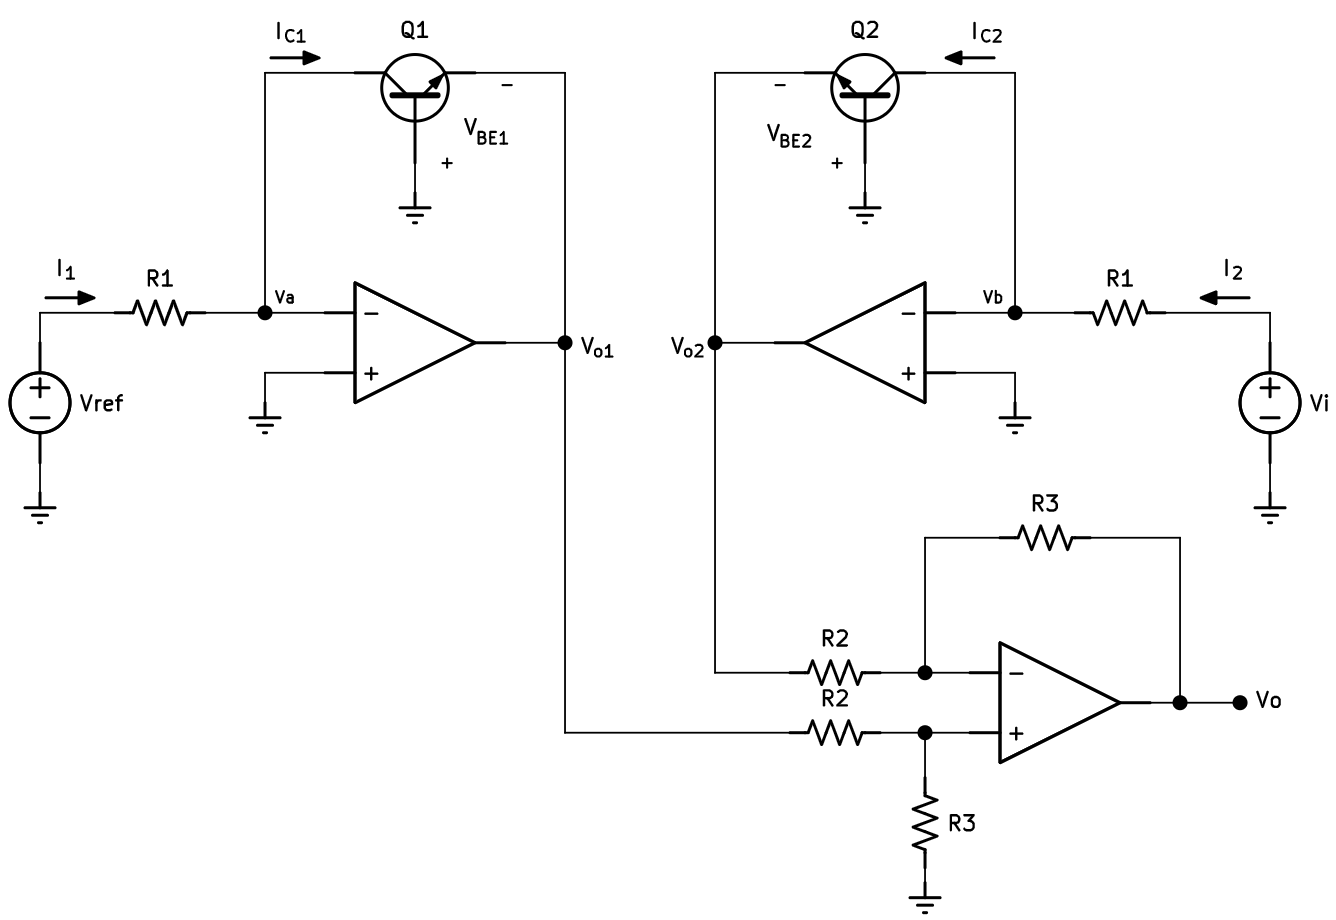
\includegraphics[scale=0.6]{log_amp1}
		\caption{Amplificador logarítmico mejorado}
		\label{fig:log_amp1}
	\end{figure}
	
	Con base en el análisis efectuado anteriormente es posible determinar rápidamente los voltajes $V_{o1}$ y $V_{o2}$, es decir
	\begin{align}
		V_{o1} = - V_T \ln \left( \frac{V_{ref}}{R_1I_S} \right)\\
		V_{o2} = - V_T \ln \left( \frac{V_i}{R_1I_S} \right)
	\end{align}
	Las salidas de los amplificadores logarítmicos están conectados a un amplificador diferencial, en cuanto a este amplificador sabemos que la salida $Vo$ es:
	
	\begin{align}
		V_o = \frac{R_3}{R_2}(V_{o1} - V_{o2})
	\end{align}
	
	La sustitución de las ecuaciones (8) y (9) en (10) produce
	\begin{align}
		V_o &= \frac{R_3}{R_2} \left[ - V_T \ln \left( \frac{V_{ref}}{R_1I_S} \right) + V_T \ln \left( \frac{V_i}{R_1I_S} \right) \right]\nonumber\\
		&= V_T \frac{R_3}{R_2} \left[ \ln \left( \frac{V_i}{R_1I_S} \right) - V_T \ln \left( \frac{V_{ref}}{R_1I_S} \right)  \right]\nonumber
	\end{align}
	\begin{align}
		V_o = V_T \frac{R_3}{R_2} \ln \left( \frac{V_i}{V_{ref}} \right)
	\end{align}

	Realizaremos un cambio de base con el fin de expresar el voltaje de salida en términos de logaritmo en base 10. Recordemos que
	\begin{tcolorbox}[colback=red!5!white,colframe=red!75!black,width=(\linewidth+0.45cm)]
		\begin{equation}
			\log_{b}N = \frac{\log_{a}N}{\log_{a}b}
		\end{equation}
	\end{tcolorbox}	

	Donde 
	\begin{subequations}
		\begin{align}
			b &= e\\
			N &= \frac{V_i}{V_{ref}}\\
			a &= 10
		\end{align}
	\end{subequations}

	Así
	\begin{align}
		\log_{e}\left( \frac{V_i}{V_{ref}} \right) = \frac{ \log_{10}\left( \frac{V_i}{V_{ref}} \right) }{ \log_{10}e } = \frac{ \log_{10}\left( \frac{V_i}{V_{ref}} \right) }{0.4343}
	\end{align}
	Para el amplificador logarítmico de la figura 2, asumiendo que $Q_1$ y $Q_2$ son transistores emparejados. El objetivo es encontrar los valores de $R_2$ Y $R_3$ de tal manera que el voltaje de salida está dado por
	\begin{align}
		V_o = 1.0\, \log _{10}\left( \frac{V_i}{V_{ref}} \right)\nonumber
	\end{align}
	
	Sustituimos la ecuación (14) en (11)
	\begin{align}
		V_o = 2.3V_T \frac{R_3}{R_2} \log_{10} \left( \frac{V_i}{V_{ref}} \right)
	\end{align}
	
	\noindent \textbf{Análisis de sensibilidad}\\
	En el diseño de cualquier circuito electrónico, la tolerancia en los valores de los componentes, así como los voltajes y corrientes de referencia pueden causar una desviación sobre la salida deseada del sistema. Sin embargo, la desviación de la salida del sistema debido a la variación de cada una de sus entradas es diferente. La salida puede llegar a ser más sensible a ciertas entradas que otras.
	
	El análisis de sensibilidad es el estudio de cómo un cierto sistema reacciona reacciona a sus entradas. Es una técnica de análisis para variables que cambian sistemáticamente dentro de un modelo y determinar los efectos de tales cambios en su salida.
	Debido a la tolerancia en los valores de los componentes, como resistores, capacitores, inductores, e incluso voltaje y corrientes de referencia, el análisis de sensibilidad es una poderosa técnica usada en el diseño de circuitos. Ayuda a determinar el efecto de cada tolerancia de entrada dentro del sistema y su efecto sobre el rendimiento general del modelo. la función de sensibilidad clásica se define como 
	
	\begin{tcolorbox}[colback=red!5!white,colframe=red!75!black,width=(\linewidth+0.45cm)]
		\begin{equation}
			\scalebox{1.5}{S}_x^{y} = \frac{\partial y}{\partial x} \frac{x}{y}
		\end{equation}
	\end{tcolorbox}

	$x$ representa el valor de los componentes tales como resistores , capacitores, inductores, referencias de voltaje, etc., $y$ representa el parámetro de salida de interés como la frecuencia, fase, voltaje de salida o corriente de salida.. el resultado de la sensibilidad determina el cambio por unidad en $y$ debido a un cambio por unidad en $x$.
	
	Para determinar qué tanto afecta al sistema cualquier cambio en la temperatura podemos escribir la siguiente ecuación
	
	\begin{align}
		\scalebox{1.8}{S}_{V_T}^{V_o} = \frac{\partial V_o}{\partial V_T} \frac{V_T}{V_o}
	\end{align}

	Donde
	\begin{align}
		\frac{\partial V_o}{\partial V_T} = \frac{\partial}{\partial V_T}\left( 2.3V_T \frac{R_3}{R_2} \log_{10} \left(\frac{V_i}{V_{ref}}\right) \right) = 2.3V_T \frac{R_3}{R_2}\log_{10}\left( \frac{V_i}{V_{ref}} \right)
	\end{align}

	Así
	\begin{align}
		\scalebox{1.8}{S}_{V_T}^{V_o} = 2.3V_T \frac{R_3}{R_2}\log_{10}\left( \frac{V_i}{V_{ref}} \right) \frac{V_T}{ 2.3V_T \frac{R_3}{R_2} \log_{10} \left( \frac{V_i}{V_{ref}} \right) } = V_T
	\end{align}

	Recordemos que $V_T$, (el voltaje térmico) está dado por
	\begin{align}
		V_T = \frac{kT}{q}
	\end{align}
	
	\newpage
	Donde:\\
	$k$ = la contante de Boltzmann, $ = 8.62 \times 10^{-5} \frac{eV}{K}$\\
	$T$ =  la temperatura absoluta en kelvins $=273.15 + C^{\circ} $\\
	$q$ = la magnitud de la carga eléctrica $= 1.60 \times 10^{-19}$ coulomb \\
	
	A una temperatura ambiente de $25^{\circ}C$ el voltaje térmico será de
	\begin{align}
		V_T = \frac{kT}{q} = \frac{(8.62 \times 10^{-4} eV/K)(273.15 + 25)K}{1.602 \times 10^{-19} C} = 160.6283 \times 10^{15} \frac{eV}{C}
	\end{align}

	Sin embargo, $1C = 6.24\times 10^{18}e$, así
	\begin{align}
		V_T = \left( 160.6283 \times 10^{15} \frac{eV}{C} \right) \left( \frac{1C}{6.24 \times 10^{18}\,e} \right) \simeq 0.0258 \, V = 25.8 \,mV\nonumber
	\end{align}

	Para hacer que la ecuación (15) sea igual a
	\begin{align}
		V_o = 1.0 \log_{10} \left( \frac{V_i}{V_{ref}} \right)\nonumber
	\end{align}
	
	tenemos que hacer que el término constante $2.3V_T \frac{R_3}{R_2}$ sea igual a $1$, por lo tanto:
	\begin{align}
		2.3V_T \frac{R_3}{R_2} = 1\nonumber\\
		\frac{R_3}{R_2} = 16.852\nonumber\\
		R_3 = 16.852R_2
	\end{align}
	
\end{document} 

	
